%!TEX root = ../main.tex
\section{Benchmark Design} 
In this section, we first introduce the design goals of \sys benchmark for table discovery tasks, and then present how to generate the \sys benchmark consisting of datasets, queries and ground truth.

\subsection{Design Goals}
We design the table discovery benchmark by the 
benchmark design criteria proposed by Jim Gray.

\noindent\textbf{Relevance.}
The benchmark covers a wide range of table discovery characteristics. First, in terms of the data lake, we incorporate 4 lakes with size ranging from 10GB to 1TB, and with column number ranging from \cc{1 million} to 10 million. Second, in terms of the queries, with the help of much human efforts, we create and label more than 10 thousand table queries that cover various query characteristics, including column semantic, column overlapping, column size, etc.



\noindent\textbf{Scalability.} The benchmark involves much larger data lakes than existing data lakes for table discovery. The data lake size should be considered from two aspects. One is the normal total storage size that is highly related  to the average table size  and the number of tables. The other is the number of total columns because almost all table discovery algorithms build index and search over a large number of columns.  \sys involves up to 1 TB data lake and 10 million columns, which is sufficient enough to evaluate the scalability.




\noindent\textbf{Simplicity.} The benchmark designs easy-to-use APIs to support table discovery in data lakes. Users can simply leverage few lines of codes to query our benchmark datasets using different algorithms and compare with them.
\cc{seems limited}





\begin{figure}[h]
	\centering
	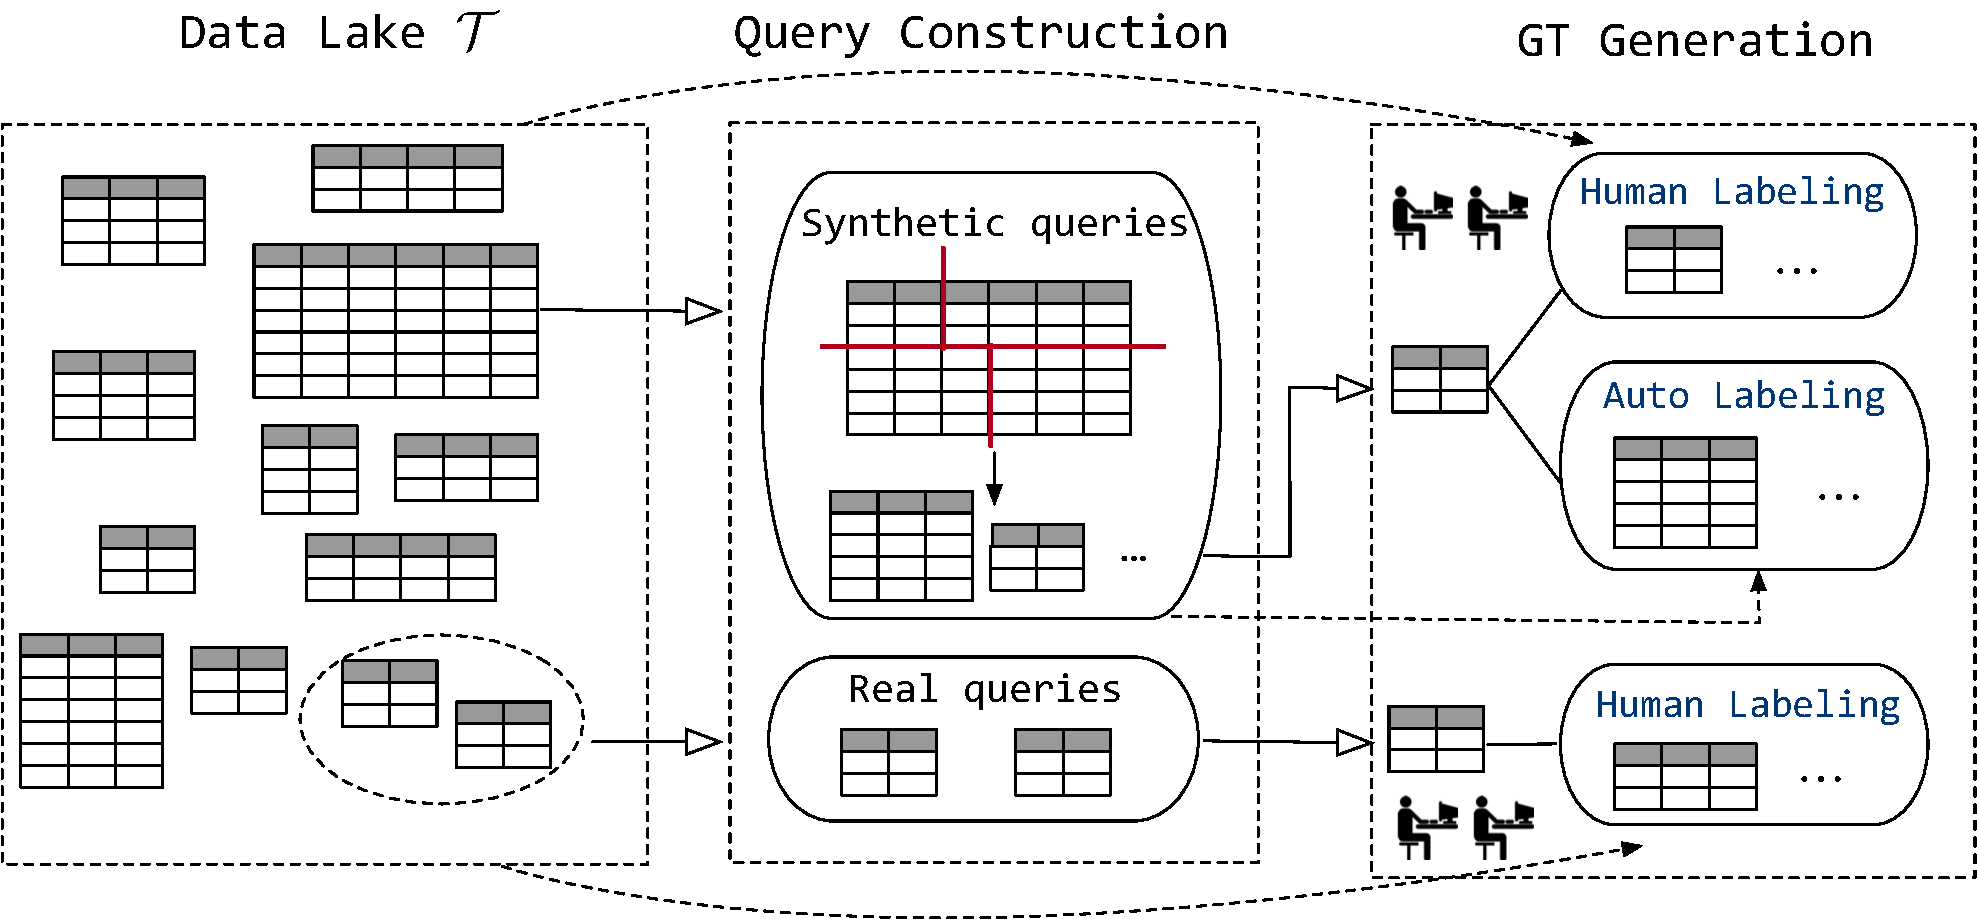
\includegraphics[width=1\linewidth]{fig/benchmark.pdf}
	\caption{Overview of \sys Construction.}
	\label{fig:benchmark}
\end{figure}



\subsection{Benchmark Overview}
In this subsection, we overview the pipeline of our benchmark design. Overall, as shown in Figure~\ref{fig:benchmark}, we first collect the datasets, then construct queries and generate ground truth for these queries. Finally, we implement various table discovery algorithms, analyze their performance from multiple perspectives, and design easy-to-use APIs.

\noindent\textbf{Datasets.}
We build 4 data lakes from OpenData~\cite{OpenData} and WebTable~\cite{WebTable}. For each data source, we create a small and large data lake respectively.

For OpenData~\cite{OpenData}, the original dataset contains XX tables, 

For WebTable~\cite{WebTable}, the original dataset contains XX tables, 


+ Statistics of collected datasets.

+ Clean the datasets.

+ Remove sth.

%Table~\ref{table} summarizes the statistics of collected datasets.


\noindent\textbf{Query Generation.}

+ Synthetic tables: split-based. Split large tables into small ones, which are put into the data lake, and then use some of the small ones as queries.

+ Real tables: retrieved-based. Use real tables as query tables, and directly query the data lake.


+ Classify: 

\quad\quad -- Column type (string, number, category)
 
\quad\quad -- Fake or real
  
\quad\quad -- Selectivity

\quad\quad -- Size

\noindent\textbf{Ground Truth Creation.}

+ Semi-automatic label: corresponding to fake tables. Some positive results are automatically generated, while others should be manually labeled.

+ Manually label: corresponding to real tables.

\noindent\textbf{Method Evaluation.} \cc{How to category}

+ \cc{Join/Union}

+ \cc{Schema matching}

+ Hash-based

+ Inverted index 

+ Pre-trained language model (HNSW)


\noindent\textbf{API Design}

    \begin{table*}[t]
        \centering
        \caption{Table Discovery Methods.}
        \begin{tabular}{|c|c|c|c|c|cccc|}
            \hline
            \multirow{2}{1cm}{\textbf{Methods}} & \multirow{2}{0.6cm}{\textbf{Task}} & \multirow{2}{0.8cm}{\textbf{Index}} & \multirow{2}{1.6cm}{\textbf{Embedding}} & \multicolumn{2}{c}{\textbf{Offline Process}} & \multicolumn{2}{c|}{\textbf{Online Process}} \\
            &&&&Time Comp.    & Space Comp. & Time Comp. & Space Comp. \\ 
            \hline
            \josie~\cite{Josie} & J & Inv. index & \XSolidBrush  & O$(\cellvaluenum + \rawtokennum \log \rawtokennum)$         & O$(\rawtokennum)$                   & O$(\positinglistlen log \positinglistlen)$         & O$(\positinglistlen)$    \\
            \hline
            \lsh~\cite{LshEn} & J & LSH & \XSolidBrush& O$(\columnnum)$        & O$(\columnnum \times \minhashlen)$                   & O$(\querycolumnnum)$                & O$(\querycolumnnum \times \minhashlen)$  \\
            \hline
            \pex~\cite{Pexeso} & J &  Inv. index& \Checkmark  & O$(\rawtokennum)$        & O$(\rawtokennum)$                   & O$(\querycellvalue + \log \querycellvalue \times \log \rawtokennum)$                & O$(\querycellvalue)$     \\
            \hline
            \deepjoin~\cite{DeepJoin} & J & HNSW & \Checkmark & O$(\columnnum)$         & O$(\columnnum)$                   & O$(\log \columnnum)$                & O$(\columnnum)$  \\
            \hline
             \tus~\cite{TUS} & U & LSH & \Checkmark  & O$(\cellvaluenum + \columnnum)$         & O$(\columnnum \times \minhashlen)$    & O$(\querycolumnnum)$               &  O$(\querycolumnnum \times \minhashlen)$     \\
            \hline
            \dlll~\cite{D3L} & U & LSH & \Checkmark& O$(\cellvaluenum + \columnnum)$          & O$(\columnnum)$                   & O$(\querycolumnnum \times \dlllneighbornnum)$                & O($\querycolumnnum$)      \\
            \hline
            \starmie~\cite{Starmie} & U & HNSW & \Checkmark & O$(\columnnum)$         & O$(\columnnum)$                   & O$(\log \columnnum)$                & O$(\columnnum)$   \\
            \hline
            \santos~\cite{Santos} & U & Inv. index & \XSolidBrush & O$(\rawtokennum)$         & O$(\rawtokennum \times \columnnum {\averagetargetcolumnnum}^2)$    & O$(\querycellvalue + \santosneighbornnum)$               & O$(\querycellvalue)$  \\
            \hline
            \frt~\cite{Frt12} & J \& U & \XSolidBrush & \XSolidBrush &  O$(\columnnum)$        & O$(\columnnum)$    & O$( \tablenum \times {(\querycolumnnum + \averagetargettuplenum)}^3)$               & O$({\averagetargettuplenum}^2)$    \\
            \hline
            \infogather~\cite{InfoGather} & J \& U & Inv. index & \XSolidBrush & O$(\columnnum^2)$   & O$(\columnnum^2)$    & O$(\querycolumnnum \times \inforneighbornnum \log \inforneighbornnum)$              & O$(\inforneighbornnum )$   \\
            \hline
            \aurum~\cite{Aurum} & J \& U & LSH & \Checkmark  & O$(\columnnum)$         & O$(\columnnum)$                   & O$(\log \columnnum)$                & O$(\columnnum)$   \\
            \hline
            Pretrain-based Method~\cite{} & U & HNSW & \Checkmark   & O$(\columnnum)$         & O$(\columnnum)$                   & O$(\log \columnnum)$                & O$(\columnnum)$ \\
            \hline
        \end{tabular}
        \label{table:methods}
        
    \end{table*}

\begin{table*}[!ht]
	\centering
	\caption{The Meaning of Different Symbols.}
	\begin{tabular}{cc}
		\hline
		Symbol & Meaning \\ \hline
		$\mathcal{B}$ & Number of columns in the query table $\qtable$  \\
		$\mathcal{N}$ &The total number of columns in all tables in the data lake $\lake$ \\
		$\mathcal{K}$ & The number of non-distinct cell values in all tables in the data lake $\lake$   \\
		$\mathcal{R}$ &The number of distinct cell values in all tables in the data lake $\lake$ \\
		$\mid \mathcal{T} \mid$ & Number of tables in the data lake $\lake$  \\
		$\mathcal{X}$ &The total number of tuples in all tables in the data lake $\lake$ \\
		$\mathcal{A}$ & The number of non-distinct cell values in query table $\qtable$  \\
		
		$\mathcal{L}$ & The length of positing list in \josie  \\
		$\mathcal{H}$ & The dimension of minhash vector \\
		$\mathcal{P}$ & The number of partition in \lsh\\
		$\mathcal{D}$ & The number of neighbors in \dlll\\
		$\mathcal{I}$ & The number of neighbors in \infogather\\
		$\overline{\mathcal{O}}$ & The average number of tuples in target column\\
		%


%fake方法造query:就是先选一个行和列都比较多的大表,然后随机选择num列(num为随机数),并且打乱这些列的顺序,再添加了一列随机数;竖着切成几个小表之后,再随机选择num行(num为随机数),并且打乱这些行的顺序,同时,选择横着切表之前的1/4行作为切完之后各个小表之间的overlap。

%不fake方法造query:随机抽选一些候选表出来,然后再人工抽取一些人能识别出来表格主题的表(方便后续ground truth的标注)

%fake方法定ground truth: 首先,竖着切之后,判断各个小表有没有属性重复,有的话,两个表之间视为可以join。除此之外,横着切生成的不同小表,由于它们之间一定会有overlap和属性重复,所以两两之间视为可union

%不fake方法定ground truth:根据不fake的方法造出来的query,利用一些简单的相似性判断捞出一些候选表,再进行人工标注

	
	\end{tabular}
	\label{symbol_table}
\end{table*}



